% Slides for the open-source model compatibility briefing.
% Build with tools/build_slides.sh <study-dir>; refs come from report/refs.bib.
\documentclass[aspectratio=169,11pt]{beamer}

\usetheme{Madrid}
\usecolortheme{default}
\setbeamertemplate{navigation symbols}{}
\usepackage[T1]{fontenc}
\usepackage{amsmath,amssymb}
\usepackage{booktabs}
\usepackage{array}
\usepackage{graphicx}
\usepackage[table]{xcolor}
\usepackage{tikz}
\usetikzlibrary{positioning,arrows.meta}
\usepackage[numbers]{natbib}

\definecolor{nativecol}{HTML}{0072B2}
\definecolor{genericcol}{HTML}{009E73}
\definecolor{partcol}{HTML}{E69F00}
\definecolor{unattcol}{HTML}{D55E00}
\usepackage{hyperref}
\setbeamercolor{structure}{fg=nativecol}
\setbeamerfont{caption}{size=\scriptsize}

\newcolumntype{L}[1]{>{\raggedright\arraybackslash}p{#1}}

\tikzset{
  ag/.style={draw=#1, line width=0.9pt, rounded corners=1pt, fill=#1!12,
    text=black, minimum width=3.0cm, minimum height=1.05cm, align=center}}

\title[Open-model support in coding agents]{Open-source model support in
Claude Code, Codex, and OpenCode}
\author[self-study-with-ai]{self-study-with-ai}
\date{2026-08-20}

\begin{document}

\begin{frame}
  \titlepage
  \note{One-sentence framing: a static-trace comparison of how three coding
  agents reach open-weight models through local or generic servers. No
  server was started and no model was called.}
\end{frame}

\begin{frame}{Outline}
  \tableofcontents
  \note{Four parts: the question, what servers provide, what agents commit
  to, and the synthesis matrix. Everything is anchored to pinned commits
  and documentation snapshots.}
\end{frame}

\section{Question}

\begin{frame}{Why this question exists}
  Coding agents usually assume a model of the vendor that ships them.
  Open-weight models reach those agents only through local or generic
  servers, and the support is uneven~\citep{codexRepo,opencodeRepo,%
  claudeCodeSurface}.

  \vspace{0.6em}
  \textbf{Three questions, all answered from static traces:}
  \begin{enumerate}
    \item Through which paths can each agent reach an open-weight model?
    \item What must a server provide before the path is usable?
    \item Where do accounting and tooling degrade around open models?
  \end{enumerate}
  \note{The study never runs agents or servers. Every claim is a code
  path, a documentation contract, or a labeled gap.}
\end{frame}

\begin{frame}{Study design}
  \textbf{Agents, pinned commits}~\citep{codexRepo,opencodeRepo,%
  claudeCodeSurface}:
  \begin{itemize}
    \item Codex CLI, commit \texttt{af700180}
    \item OpenCode, commit \texttt{d545d8fb} (\textsf{dev} branch)
    \item Claude Code, bundled assets at commit \texttt{c3d2e35e}
  \end{itemize}

  \vspace{0.4em}
  \textbf{Server contracts, snapshots of three reference servers}:
  Ollama, LM Studio, llama.cpp.

  \vspace{0.4em}
  \textbf{Out of scope}: execution, API calls, third-party routers as
  attested behavior.
  \note{Tiers: codebase traces anchor to file:line at the pinned commits;
  docs and blog snapshots were saved at gathering time because the
  summarizer has no web access.}
\end{frame}

\section{What the servers offer}

\begin{frame}{The wire protocols, as a bar}
  \begin{center}
    \scalebox{0.60}{%
    \begin{tikzpicture}[font=\scriptsize,
      proto/.style={draw=black!70, line width=0.7pt, rounded corners=1pt,
        fill=black!5, align=center, minimum width=3.85cm, minimum height=0.95cm,
        inner sep=2.5pt, text=black},
      reqlab/.style={draw=black!40, line width=0.5pt, rounded corners=1pt,
        align=center, minimum width=3.85cm, minimum height=0.85cm,
        inner sep=2.5pt, text=black},
      chip/.style={rounded corners=1pt, align=center, minimum width=3.85cm,
        minimum height=0.85cm, inner sep=2.5pt, text=black},
      rowhead/.style={draw=black!50, line width=0.5pt, rounded corners=1pt,
        fill=black!5, align=center, minimum width=2.3cm, inner sep=2.5pt,
        text=black},
      arr/.style={-{Stealth[length=1.8mm]}, draw=black!60, line width=0.5pt}]
      \node[proto] (p1) at (0,0) {\textbf{Chat completions}\\ plus tool calls};
      \node[proto] (p2) at (4.25,0) {\textbf{Responses API}\\ (OpenAI)};
      \node[proto] (p3) at (8.5,0) {\textbf{Anthropic}\\ \path{/v1/messages}};
      \node[reqlab, fill=genericcol!14] (oc) at (0,1.75) {\textcolor{genericcol}{OpenCode} accepts any\\ chat-completions shape};
      \node[reqlab, fill=nativecol!14] (cx) at (4.25,1.75) {\textcolor{nativecol}{Codex} pins Responses;\\ \path{chat} is a hard error};
      \node[reqlab, fill=unattcol!14] at (8.5,1.75) {\textcolor{unattcol}{Claude Code}: Anthropic\\ protocol only, as attested};
      \draw[arr] (oc.south) -- (p1.north);
      \draw[arr] (cx.south) -- (p2.north);
      \node[rowhead] at (-3.0,-1.4) {Ollama\\ 2024 snapshot};
      \node[chip, fill=partcol!16] at (0,-1.4) {partial: chat yes, tools\\ listed as future};
      \node[chip, fill=black!7] at (4.25,-1.4) {absent: not in snapshot};
      \node[chip, fill=black!7] at (8.5,-1.4) {absent: not in snapshot};
      \node[rowhead] at (-3.0,-2.5) {LM Studio\\ docs mirror};
      \node[chip, fill=genericcol!14] at (0,-2.5) {supported: tools on chat\\ completions; no parallel flag};
      \node[chip, fill=partcol!16] at (4.25,-2.5) {partial: streaming, effort,\\ prior state, remote MCP only};
      \node[chip, fill=black!7] at (8.5,-2.5) {named only: shape\\ undocumented};
      \node[rowhead] at (-3.0,-3.6) {llama.cpp\\ reference server};
      \node[chip, fill=genericcol!14] at (0,-3.6) {supported: tools via\\ jinja templates, JSON schema};
      \node[chip, fill=partcol!16] at (4.25,-3.6) {partial: documented as a\\ converter to chat completions};
      \node[chip, fill=genericcol!14] at (8.5,-3.6) {supported:\\ \path{/v1/messages} documented};
    \end{tikzpicture}}
  \end{center}
  \note{Read it as a bar to clear. Top row is what each agent commits
  to on the wire; the grid is what the reference servers document. The
  Responses column, which Codex needs, is the youngest surface
  everywhere. Every status is written in its chip.}
\end{frame}

\begin{frame}{Two readings of the bar}
  \begin{enumerate}
    \item \textbf{Practical minimum}: chat completions with tool
    calling. Structured output support is uneven across servers.
    \item \textbf{The Responses surface is young}: documented as partial
    on every server that documents it at
    all~\citep{ollamaCompatDocs,lmstudioApiDocs,llamaCppServerDocs}.
  \end{enumerate}

  \vspace{0.6em}
  Also relevant later: llama.cpp documents an Anthropic-shaped
  \path{/v1/messages} route, and LM Studio names an Anthropic-compatible
  surface.
  \note{Both facts become important in the Claude Code frame. They are the
  closest attested Anthropic-shaped surfaces, and neither is verified
  against Claude Code.}
\end{frame}

\section{What the agents commit to}

\begin{frame}{Codex: a first-class Responses path, with caveats}
  \begin{itemize}
    \item Native providers for Ollama and LM Studio speak the Responses
    API to \path{/v1/responses}~\citep{codexRepo}.
    \item Version gate on Ollama: refuses reported versions below
    \texttt{0.13.4}, with exceptions for dev builds and unreported or
    unparsable versions.
    \item Defaults are catalog misses (\path{gpt-oss:20b},
    \path{openai/gpt-oss-20b}), so a fallback-metadata path applies
    unless a catalog refresh decodes a richer listing.
    \item Generic servers reach the wire protocol only via
    \path{model_providers} config, Responses wire
    only~\citep{codexRepo}.
  \end{itemize}
  \note{Caveat carried from the report: Codex also drops apply_patch from
  tools when the server lacks structured output, and nothing in this trace
  was executed.}
\end{frame}

\begin{frame}{OpenCode: generic compatibility, permissive defaults}
  \begin{itemize}
    \item The path is generic: \path{@ai-sdk/openai-compatible} with
    \path{baseURL} and \path{apiKey}; packages install at runtime, with
    \path{file://} local overrides~\citep{opencodeRepo}.
    \item Model catalog: hosted \path{models.opencode.ai} by default, a
    local catalog file wins if present, three environment variables
    override~\citep{opencodeRepo}.
    \item Degradation defaults: context limit \texttt{0} disables
    auto-compaction; output limit \texttt{0} becomes a \texttt{32,000}
    token cap; tokens are estimated as characters divided by four.
    \item Unknown model IDs fail hard with fuzzy suggestions; tools ride
    along unconditionally in the request.
  \end{itemize}
  \note{The same defaults that make an open model loadable also make token
  accounting wrong unless the user fills in the limits.}
\end{frame}

\begin{frame}{Claude Code: no documented surface, and a gray zone}
  \begin{itemize}
    \item Every documented model example is an Anthropic model: IDs or
    names prefixed or namespaced \texttt{anthropic.}, plus Bedrock
    inference-profile ARNs~\citep{claudeCodeModelDocs,claudeCodeBedrockDocs}.
    \item No documented Ollama, LM Studio, or llama.cpp
    surface~\citep{ollamaCompatDocs,lmstudioApiDocs,llamaCppServerDocs}.
    \item The gray zone sits in unverified conditions: a base-URL
    override, a custom model option string that is passed through
    verbatim, and a max-context setting with precise preconditions.
    \item \textsf{claude-code-router} is an existence proof that users
    route; its behavior is not attested here~\citep{claudeCodeRouterContext}.
  \end{itemize}
  \note{Negative-scope claim. The report states only what the docs do and
  do not attest, not what the loader does at runtime.}
\end{frame}

\section{Synthesis}

\begin{frame}{Support as a graph}
  \begin{center}
    \scalebox{0.72}{%
    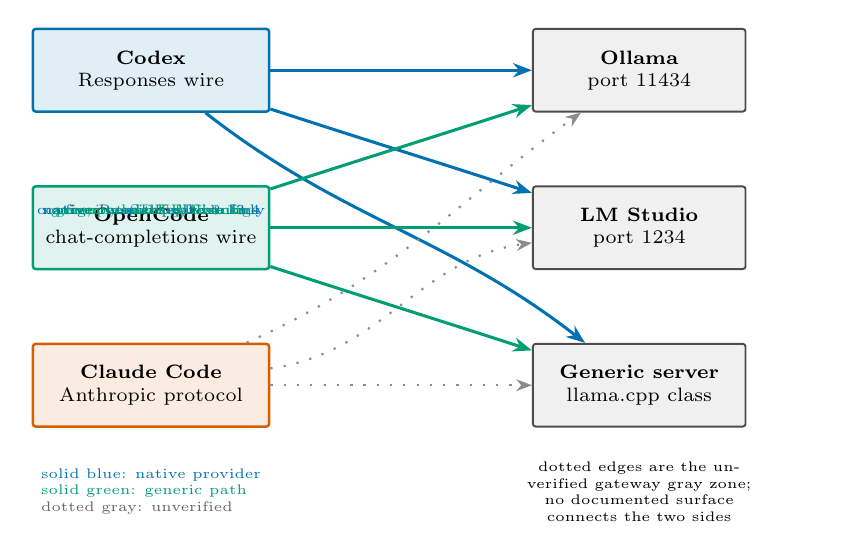
\begin{tikzpicture}[font=\scriptsize,
      sv/.style={draw=black!70, line width=0.7pt, rounded corners=1pt,
        fill=black!6, text=black, minimum width=2.7cm, minimum height=1.05cm,
        align=center},
      nat/.style={-{Stealth[length=2.4mm]}, line width=1.1pt, nativecol},
      gen/.style={-{Stealth[length=2.4mm]}, line width=1.1pt, genericcol},
      unv/.style={-{Stealth[length=2mm]}, line width=0.8pt, black!45, loosely dotted}]
      \node[ag=nativecol] (cx) at (0, 2.0) {\textbf{Codex}\\ Responses wire};
      \node[ag=genericcol] (oc) at (0, 0.0) {\textbf{OpenCode}\\ chat-completions wire};
      \node[ag=unattcol] (cc) at (0,-2.0) {\textbf{Claude Code}\\ Anthropic protocol};
      \node[sv] (ol) at (6.2, 2.0) {\textbf{Ollama}\\ port 11434};
      \node[sv] (lm) at (6.2, 0.0) {\textbf{LM Studio}\\ port 1234};
      \node[sv] (gn) at (6.2,-2.0) {\textbf{Generic server}\\ llama.cpp class};
      \draw[nat] (cx) to[out=0, in=180] (ol)
        node[sloped, midway, above, font=\tiny, text=nativecol, pos=0.5] {native; version gate 0.13.4};
      \draw[nat] (cx) to[out=-18, in=162] (lm)
        node[sloped, midway, above, font=\tiny, text=nativecol, pos=0.52] {native; model pull via lms};
      \draw[nat] (cx) to[out=-38, in=142] (gn)
        node[sloped, midway, above, font=\tiny, text=nativecol, pos=0.58] {config; Responses wire only};
      \draw[gen] (oc) to[out=18, in=198] (ol)
        node[sloped, midway, above, font=\tiny, text=genericcol, pos=0.48] {generic; baseURL config};
      \draw[gen] (oc) to[out=0, in=180] (lm)
        node[sloped, midway, above, font=\tiny, text=genericcol, pos=0.5] {generic; catalog fixture};
      \draw[gen] (oc) to[out=-18, in=162] (gn)
        node[sloped, midway, above, font=\tiny, text=genericcol, pos=0.52] {compat-SDK fallback};
      \draw[unv] (cc) to[out=24, in=216] (ol);
      \draw[unv] (cc) to[out=8, in=188] (lm);
      \draw[unv] (cc) to[out=0, in=180] (gn);
      \node[align=center, font=\tiny, text width=4.6cm] at (6.2,-3.35)
        {dotted edges are the unverified gateway gray zone;\\ no documented surface connects the two sides};
      \node[align=left, font=\tiny] at (0,-3.35)
        {\textcolor{nativecol}{solid blue: native provider}\\
         \textcolor{genericcol}{solid green: generic path}\\
         \textcolor{black!60}{dotted gray: unverified}};
    \end{tikzpicture}}
  \end{center}
  \note{Same matrix as the report table, drawn as a graph. Edge styles
  encode tier plus certainty; the labels repeat both, so the figure reads
  in grayscale too.}
\end{frame}

\begin{frame}{The directional claim}
  \textbf{Compatibility with open models is decided by the wire protocol
  an agent commits to.}

  \vspace{0.6em}
  \begin{itemize}
    \item \textcolor{nativecol}{Codex} pinned to Responses and built
    native plumbing for two local servers, accepting the patch-tool loss.
    \item \textcolor{genericcol}{OpenCode} pinned to nothing and accepts
    anything chat-completions-shaped, accepting misbehaving defaults.
    \item \textcolor{unattcol}{Claude Code} commits to Anthropic's stack
    and leaves the rest to an unattested gateway.
  \end{itemize}

  \vspace{0.6em}
  Each bet has a matching price, paid in a different currency.
  \note{This is the one claim the whole briefing builds toward. Every
  bullet traces to the agent findings frames.}
\end{frame}

\begin{frame}{Limitations}
  \begin{itemize}
    \item \textbf{Nothing was executed.} No server started, no model
    called; every statement is a code path or a documentation contract.
    \item \textbf{Snapshots can lag.} The Ollama post is from 2024; LM
    Studio live docs were unreachable, so we cite the GitHub mirror.
    \item \textbf{Two hedges.} Codex fallback metadata (including the
    272k claim) and OpenCode's compaction paths are reported with
    explicit uncertainty because the traces leave open cells.
    \item \textbf{vLLM absent}: its docs moved and could not be
    relocated honestly.
  \end{itemize}
  \note{The hedges exist because the review stage demanded that any open
  cell stays open in the text.}
\end{frame}

\begin{frame}{Takeaways}
  \begin{enumerate}
    \item The cheapest entry point for open models today is
    \textcolor{genericcol}{OpenCode's} generic path: configure a base URL
    and fill in limits, or accept wrong accounting.
    \item The most integrated entry point is \textcolor{nativecol}{Codex},
    at the price of the Responses bet on server-side adoption.
    \item For \textcolor{unattcol}{Claude Code}, open-model support
    currently lives in the community router, not in the product.
  \end{enumerate}

  \vspace{0.6em}
  Full report: \texttt{report/main.pdf}. Evidence: pinned commits,
  registry, snapshots.
  \note{End the talk on the directional claim and the three currencies.}
\end{frame}

\begin{frame}[allowframebreaks]{References}
  \footnotesize
  \bibliographystyle{plainnat}
  \bibliography{refs}
  \note{All entries carry pinned commits or snapshot provenance.}
\end{frame}

\appendix

\begin{frame}{Backup: degradation constants}
  \textbf{Codex fallback-metadata gaps}~\citep{codexRepo}:
  \begin{itemize}
    \item \path{apply_patch} is not registered under fallback metadata
    unless the server advertises structured output.
    \item The 272,000-token context claim is unverified for the
    catalog-miss path.
  \end{itemize}
  \textbf{OpenCode defaults}~\citep{opencodeRepo}:
  \begin{itemize}
    \item \path{context} $=0$ disables auto-compaction entirely.
    \item \path{output} $=0$ becomes \path{OUTPUT_TOKEN_MAX}$=32000$.
    \item token estimate: \path{characters / 4}.
  \end{itemize}
\end{frame}

\begin{frame}{Backup: gray-zone conditions}
  \begin{itemize}
    \item \path{ANTHROPIC_BASE_URL}: documented, wire shape unattested.
    \item \path{ANTHROPIC_CUSTOM_MODEL_OPTION}: ``you can use any string
    your API endpoint accepts''~\citep{claudeCodeModelDocs}.
    \item \path{CLAUDE_CODE_MAX_CONTEXT_TOKENS}: applies only when the
    model name does not start with \texttt{claude-}, is not a
    \texttt{[1m]} variant, and does not resolve to a Claude
    model~\citep{claudeCodeModelDocs}.
  \end{itemize}
\end{frame}

\begin{frame}{Backup: open gaps from the gap register}
  \begin{enumerate}
    \item Codex catalog-refresh behavior against real LM Studio and
    Ollama listings.
    \item OpenCode compaction path selection (v1 vs. v2) at zero context
    limit.
    \item Claude Code gateway wire shape behind a base-URL override.
    \item LM Studio Responses feature coverage beyond the documented
    subset.
  \end{enumerate}
\end{frame}

\end{document}
